\documentclass[11pt,titlepage]{article}

\usepackage[margin=1.5in]{geometry}
\usepackage{amsmath}
\usepackage{caption}
\usepackage{tablefootnote}
\usepackage{algorithm2e}
\usepackage{amssymb}
\usepackage{bbm}
\usepackage{derivative}
\usepackage{float}
\usepackage{graphicx}
\usepackage{hyperref}
\usepackage{listings}
\usepackage{parskip}
\usepackage{xcolor}

\definecolor{codegreen}{rgb}{0,0.6,0}
\definecolor{codegray}{rgb}{0.5,0.5,0.5}
\definecolor{codepurple}{rgb}{0.58,0,0.82}
\definecolor{backcolour}{rgb}{0.95,0.95,0.92}

\lstdefinestyle{mystyle}{
    backgroundcolor=\color{backcolour},
    commentstyle=\color{codegreen},
    keywordstyle=\color{magenta},
    numberstyle=\tiny\color{codegray},
    stringstyle=\color{codepurple},
    basicstyle=\ttfamily\footnotesize,
    breakatwhitespace=false,
    breaklines=true,
    captionpos=b,
    keepspaces=true,
    numbers=left,
    numbersep=2pt,
    showspaces=false,
    showstringspaces=false,
    showtabs=false,
    tabsize=2
}

\lstset{style=mystyle}

\newcommand{\HRule}{\rule{\linewidth}{0.5mm}}
\title{
    \HRule\\[0.3cm]
    MA5232: Assignment 1
    \HRule\\[0.3cm]
}
\author{Rahul Venkatesh}

\begin{document}
{\let\newpage\relax\maketitle}
\tableofcontents

\section{Problem}
Consider the following 3D equation defined on $\Omega = (-1, 1) \times (-1, 1) \times (-1, 1)$.
\begin{align*}
    \pdv{F_1}{x} &= \sigma (\frac{1}{6} \Sigma F_i - F_1) \\[1em]
    -\pdv{F_2}{x} &= \sigma (\frac{1}{6} \Sigma F_i - F_2) \\[1em]
    \pdv{F_3}{y} &= \sigma (\frac{1}{6} \Sigma F_i - F_3) \\[1em]
    -\pdv{F_4}{y} &= \sigma (\frac{1}{6} \Sigma F_i - F_4) \\[1em]
    \pdv{F_5}{z} &= \sigma (\frac{1}{6} \Sigma F_i - F_5) \\[1em]
    -\pdv{F_6}{z} &= \sigma (\frac{1}{6} \Sigma F_i - F_6)
\end{align*}

The boundary conditions are
\begin{align*}
    F_1(-1, y, z) &= F_b(y, z) \\
    F_3(x, -1, z) &= F_b(x, z) \\
    F_5(x, y, -1) &= F_b(x, y) \\
    F_2(1, y, z) &= 0 \\
    F_4(x, 1, z) &= 0 \\
    F_6(x, y, 1) &= 0
\end{align*}

where

$$
F_b(p, q) =
\begin{cases}
    1 & \text{if } |p| \le 0.2 \text{ and } |q| \le 0.2 \\
    0 & \text{otherwise}
\end{cases}
$$

Solve the system of equations numerically for $\sigma  = 0.1, 1, 10, 100$.

\newpage
\section{Methods}

Iterative methods are used to solve the system of PDEs. Starting with an initial guess of the solution, in each
iteration, the solution is improved using the solution from the previous iteration. The process is continued until the
solution converges. The convergence criterion is that the computed residuals are as little as the set threshold.


The derivatives are approximated with finite differences, and the interval $\Omega$ is discretized into a uniform grid
with $\Delta x = \Delta y = \Delta z = \frac{2}{N}$ where $N$ is the number of cells.
Consider point $p_i = -1 + i\frac{\Delta p}{2}$.
The 1-indexed $cell[i, j, k]$ represents the region
$$
T_{ijk} = [x_i - \frac{\Delta x}{2}, x_i + \frac{\Delta x}{2}] \times
[y_i - \frac{\Delta y}{2}, y_i + \frac{\Delta y}{2}] \times
[z_i - \frac{\Delta z}{2}, z_i + \frac{\Delta z}{2}]
$$
For simplicity, rename the functions $F_1$ through $F_6$ as $a, b, c, d, e$ and $f$ respectively. Approximate $a(x, y,
z)$ in the region $cell[i, j, k]$ as
$$A_{ijk} \approx \frac{1}{|T_{ijk}|}\int_{T_{ijk}} a(x, y, z)dxdydz$$

Similarly, define approximations of the other 5 functions.

Obtain the following system of linear equations using finite differences to approximate the partial derivatives.

\begin{align*}
    \frac{A_{ijk} - A_{i-1,jk}}{\Delta x} &=
    \sigma [\frac{1}{6}(A_{ijk} + B_{ijk} + C_{ijk} + D_{ijk} + E_{ijk} + F_{ijk}) - A_{ijk}] \\
    \frac{B_{ijk} - B_{i+1,jk}}{\Delta x} &=
    \sigma [\frac{1}{6}(A_{ijk} + B_{ijk} + C_{ijk} + D_{ijk} + E_{ijk} + F_{ijk}) - B_{ijk}] \\
    \frac{C_{ijk} - C_{i,j-1,k}}{\Delta y} &=
    \sigma [\frac{1}{6}(A_{ijk} + B_{ijk} + C_{ijk} + D_{ijk} + E_{ijk} + F_{ijk}) - C_{ijk}] \\
    \frac{D_{ijk} - D_{i,j+1,k}}{\Delta y} &=
    \sigma [\frac{1}{6}(A_{ijk} + B_{ijk} + C_{ijk} + D_{ijk} + E_{ijk} + F_{ijk}) - D_{ijk}] \\
    \frac{E_{ijk} - E_{ij,k-1}}{\Delta z} &=
    \sigma [\frac{1}{6}(A_{ijk} + B_{ijk} + C_{ijk} + D_{ijk} + E_{ijk} + F_{ijk}) - E_{ijk}] \\
    \frac{F_{ijk} - F_{ij,k+1}}{\Delta z} &=
    \sigma [\frac{1}{6}(A_{ijk} + B_{ijk} + C_{ijk} + D_{ijk} + E_{ijk} + F_{ijk}) - F_{ijk}] \\
\end{align*}

with suitable boundary conditions by converting points in the domain into indices in the grid.


\subsection{Fixed-point Iteration (FP)}
The idea is to solve each of the six equations individually assuming the other variables are given.

\begin{align*}
    \frac{A^{(l + 1)}_{ijk} - A^{(l + 1)}_{i-1,jk}}{\Delta x} &=
    \sigma [\frac{1}{6}(A^{(l + 1)}_{ijk} + B^{(l)}_{ijk} + C^{(l)}_{ijk} + D^{(l)}_{ijk} + E^{(l)}_{ijk} +
    F^{(l)}_{ijk}) - A^{(l + 1)}_{ijk}] \\
    \frac{B^{(l + 1)}_{ijk} - B^{(l + 1)}_{i+1,jk}}{\Delta x} &=
    \sigma [\frac{1}{6}(A^{(l)}_{ijk} + B^{(l + 1)}_{ijk} + C^{(l)}_{ijk} + D^{(l)}_{ijk} + E^{(l)}_{ijk} +
    F^{(l)}_{ijk}) - B^{(l + 1)}_{ijk}] \\
\end{align*} where $A^{(l)}$ is $A$ in the $l^{\text{th}}$ iteration.

In the first equation, $A$ is computed using $B, C, D, E$ and $F$ from the previous iteration. Similarly, in the
second equation, $B$ is computed using $A, C, D, E$ and $F$ from the previous iteration. One could also use latest
values computed in the current iteration. For example, in the second equation, $A^{(l + 1)}$ can be used instead of
$A^{(l)}$. The values can be updated linearly. Note that $B$ needs to be updated backwards and $A$ forwards.

The update rules follow for the rest of the matrices in $y$ and $z$ dimensions.

\subsubsection{Relaxation}

Each iteration only contains six small loops (of size $N$) and matrix additions making the iterations quite fast (around
5 iterations per second). But the problem arises when $\sigma$ is large: while the individual iterations are fast,
convergence is slow. For $\sigma = 100$, after 1000 iterations, the residual was still $1.8$.

To solve this slow convergence issue, each update is relaxed with an additional term.

\begin{multline*}
    \epsilon (A^{(l + 1)}_{ijk} - A^{(l)}_{ijk}) + \frac{A^{(l + 1)}_{ijk} - A^{(l + 1)}_{i-1,jk}}{\Delta x} = \\
    \sigma [\frac{1}{6}(A^{(l + 1)}_{ijk} + B^{(l)}_{ijk} + C^{(l)}_{ijk} + D^{(l)}_{ijk} + E^{(l)}_{ijk} +
    F^{(l)}_{ijk}) - A^{(l + 1)}_{ijk}]
\end{multline*}

However, the choice of $\epsilon$ is unclear and the process may diverge with the wrong $\epsilon$.

\newpage
\subsection{Symmetric Gauss-Seidel (SGS)}

Each iteration contains two scans. The first scan is carried out in a
left-to-right, bottom-to-top, back-to-front fashion; the second scan is carried out in a right-to-left,
top-to-bottom, front-to-back fashion.

First scan:
\begin{align*}
    \frac{A^{(l + 1)}_{ijk} - A^{(l + 1)}_{i-1,jk}}{\Delta x} &=
    \sigma [\frac{1}{6}(A^{(l + 1)}_{ijk} + B^{(l + 1)}_{ijk} + C^{(l + 1)}_{ijk} + D^{(l + 1)}_{ijk} + E^{(l + 1)}_{ijk} +
    F^{(l + 1)}_{ijk}) - A^{(l + 1)}_{ijk}] \\
    \frac{B^{(l + 1)}_{ijk} - B^{(l)}_{i+1,jk}}{\Delta x} &=
    \sigma [\frac{1}{6}(A^{(l + 1)}_{ijk} + B^{(l + 1)}_{ijk} + C^{(l + 1)}_{ijk} + D^{(l + 1)}_{ijk} + E^{(l + 1)}_{ijk} +
    F^{(l + 1)}_{ijk}) - B^{(l + 1)}_{ijk}]
\end{align*}

Note that the right-hand side, in contrast to the fixed-point iteration updates, uses the values from current iteration. On
the left-hand side, $B_{i+1,jk}$ uses the previous iteration's value as it hasn't been computed in the current scan yet,
and $A_{i-1,jk}$ uses the current iteration's value which was computed in the previous step. Similarly, the second
scan will use $A_{i-1,jk}^{(l)}$ and $B_{i+1,jk}^{(l + 1)}$. Either way, they are both known values. However, the
entire right-hand side is unknown. Moving the unknowns to the left gives us the following system of linear equations.

$$
M\begin{pmatrix}
    A_{ijk}\\
    B_{ijk}\\
    C_{ijk}\\
    D_{ijk}\\
    E_{ijk}\\
F_{ijk}\end{pmatrix} = x_{ijk} = 
\begin{pmatrix}
    \frac{1}{\Delta x}A_{i-1,jk}\\
    \frac{1}{\Delta x}B_{i+1,jk}\\
    \frac{1}{\Delta y}C_{i,j-1,k}\\
    \frac{1}{\Delta y}D_{i,j+1,k}\\
    \frac{1}{\Delta z}E_{i,j,k-1}\\
    \frac{1}{\Delta z}F_{i,j,k+1}\\
\end{pmatrix}
$$

where

\begin{equation*}
\begin{split}
    M &= \begin{bmatrix} \frac{1}{\Delta x} & & & & & \\
                         & \frac{1}{\Delta x} & & & & \\
                         & & \frac{1}{\Delta y} & & & \\
                         & & & \frac{1}{\Delta y} & & \\
                         & & & & \frac{1}{\Delta z}  & \\
                         & & & & & \frac{1}{\Delta z}\\\end{bmatrix}
         + \sigma I- \frac{\sigma}{6}\mathbf{1}\mathbf{1}^T \\
      &= (\frac{1}{\Delta x} + \sigma)I - \frac{\sigma}{6}\mathbf{1}\mathbf{1}^T
\end{split}
\end{equation*}

This can be solved for each $(i, j, k)$ by computing the constant $M^{-1}$ and dot product.

\begin{lstlisting}[language=python,caption={First Scan},captionpos=b]
for i in range(1, N + 1):
    for j in range(1, N + 1):
        for k in range(1, N + 1):
            x = (N/2) * np.array([
                A[i - 1, j, k],
                B[i + 1, j, k],
                C[i, j - 1, k],
                D[i, j + 1, k],
                E[i, j, k - 1],
                F[i, j, k + 1],
            ])
            A[i, j, k], B[i, j, k], C[i, j, k], \
            D[i, j, k], E[i, j, k], F[i, j, k] = M_inv.dot(x)
\end{lstlisting}


\subsubsection{Red-Black ordering}
Although the SGS method results in a clean exact solution, the algorithm itself is
inherently sequential. Each iteration has two for-loops of size $N^3$ which makes the updates very slow (around 14
seconds per iteration) and difficult to parallelize (i.e., exploit fast matrix operations).

The idea of the \href{https://math.mit.edu/classes/18.086/2006/am62.pdf}{red-black ordering} for two-dimensional grid is to color odd grid cells ($i + j \equiv 1 \text{ (mod }2)$)
red and the even grid cells black. Since the values of the red cells only depend on the black cells and vice versa, the
first scan can update all red cells, and the second scan updates all black cells. The main advantage is that the
updates can be parallelized.

For this problem, the 3D grid can be colored using three colors: red, blue and green depending on $(i + j + k) \text{
mod }3$. However, for this problem, this scheme is exceedingly slow in convergence and also slow in each iteration due to the
$O(N^3)$ matrix for parallel update.

\subsubsection{Successive Over Relaxation (SOR)}
For large $\sigma$, the convergence is still slow: for $\sigma = 100$, after 1000 iterations, the residual was still
$0.02$. In the spirit of the Fixed-point iteration method with relaxation, a
\href{https://en.wikipedia.org/wiki/Successive_over-relaxation}{relaxation factor}, $\omega$, can be introduced over
here as well. If $\overline{A}_{ijk}^{(l + 1)}$ were the original SGS value, the relaxed SGS update would be

$$
A_{ijk}^{(l + 1)} \leftarrow  (1 - \omega) A_{ijk}^{(l)} + \omega \overline{A}_{ijk}^{(l + 1)}
$$

\newpage
\subsubsection{Optimization}
As noted earlier, SGS iterations are time-consuming. Even if SOR helps with faster convergence, just 100 iterations
takes 25 minutes. Although the algorithm is still sequential, writing in terms of matrices would be helpful as
python's \texttt{numpy} provides vectorization benefits.

In the inner most loop, only $E$ depends on the value computed by the previous for-iteration. For given $(i, j)$,
compute $E_{ijk}$ (dropping $_{ij}$ for brevity) first as

$$
E_{k} = M^{-1}_{5}[-5] x_{k}[-5] + M^{-1}_{55} E_{k-1}
$$

where $M^{-1}_{5}[-5]$ is the 5th row without the 5th column, $x_k[-5]$ is the column vector without the 5th entry (row)
and $M_{55}$ is the 5th row and 5th column. This recursion can be converted into element-wise \texttt{np.array}
multiplications and \texttt{np.cumsum}. Now, that all $E_k$ has been computed for given $(i, j)$, the other
matrices at all $k$ can be computed by one matrix multiplication as $M^{-1}X$ where $X = [x_1, x_2, \dots x_k, \dots, x_N]$.

This gives us the much needed 15x speed boost: each iteration runs under a second.

\section{Setting}
Number of points: $N = 100$; threshold of convergence: $\delta = 10^{-6}$.

\begin{table}[h]
    \centering
    \begin{tabular}{r|r|r|r|r}
        \hline
        parameter & $\sigma = 0.1$ & $\sigma = 1$ & $\sigma  = 10$ & $\sigma  = 100$ \\
        \hline
        SGS $\omega$  & 1 & 1 & 1.05 & 1.37 \\
        \hline
        FP $\epsilon$  & 0 & 0 & -3 & -40 \\
        \hline
    \end{tabular}
    \caption{Recommended settings for fast convergence}
\end{table}

\section{Results}

\begin{table}[h]
    \centering
    \begin{tabular}{r|r|r|r|r|r|r|r|r}
        \hline
        Method & \multicolumn{4}{c}{Num of iterations} & \multicolumn{4}{c}{Time (in s)} \\
               & $\sigma = 0.1$ & $\sigma = 1$ & $\sigma  = 10$ & $\sigma  = 100$
               & $\sigma = 0.1$ & $\sigma = 1$ & $\sigma  = 10$ & $\sigma  = 100$ \\

        \hline

        SGS  & 4 & 11 & 167 & 1000\tablefootnote{did not converge; residual=0.02} & 3.22 & 8.92 & 144.93 & $844.38^{1}$ \\
        \hline
        SGS with $\omega$  & 4 & 11 & 47 & 156 & 3.90 & 10.32 & 43.15 & 141.30 \\
        \hline
        FP  & 5 & 16 & 328 & 1000\tablefootnote{did not converge; residual=1.83} & 1.28 & 3.88 & 78.26 & $235.59^{2}$ \\
        \hline
        FP with $\epsilon$  & 5 & 16 & 96 & 559 & 1.22 & 3.85 & 20.14 & 121.76 \\
        \hline
    \end{tabular}
    \caption{Performance comparison of the methods}
\end{table}

\subsection{Plots}

The following pages contain the visual representation of the solution as provided by the SGS method with appropriate
relaxations. The solution provided by FP and SGS have $\text{RMSE}=0.002$ (sanity check: basically the same).

Figure \ref{fig:sgs_c} shows the residual as the method iterates. The residuals (y-axis) are represented on the
log-scale. Both methods yield similar convergence steps except the number of iterations to converge.

Figure \ref{fig:3d_1} and \ref{fig:3d_10} is a heatmap of $(A + B + C + D + E + F)$ plotted on the planes $x = 0, y =
0$ and $z = 0$.

Figure \ref{fig:sgs_0.1} through \ref{fig:sgs_100} shows the heatmaps of $A$, $B$ and $(A + B + C + D + E + F)$ but as a
2D plot instead of a 3D plot.


\begin{figure}[H]
    \centering
    \caption{Residual vs iterations for SGS}
    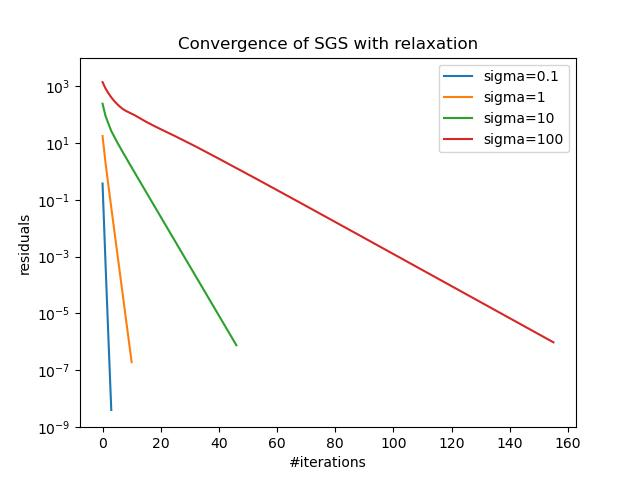
\includegraphics[scale=0.8]{img/sgs_convergence.jpg}
    \label{fig:sgs_c}
    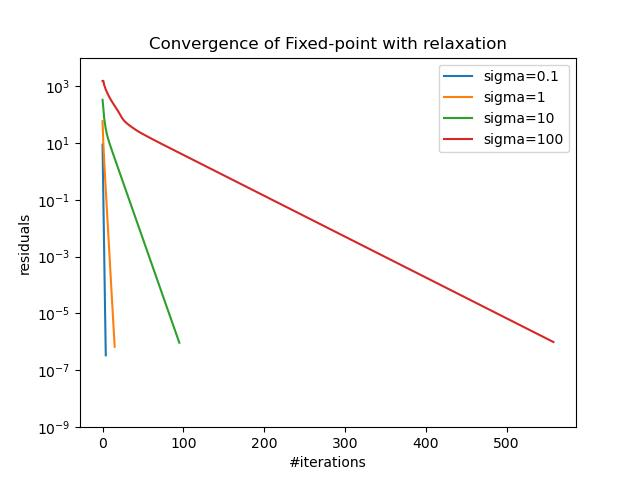
\includegraphics[scale=0.8]{img/fp_convergence.jpg}
    \label{fig:fp_c}
\end{figure}

\begin{figure}[H]
    \centering
    \caption{3D visualization of sum of $F_i$}
    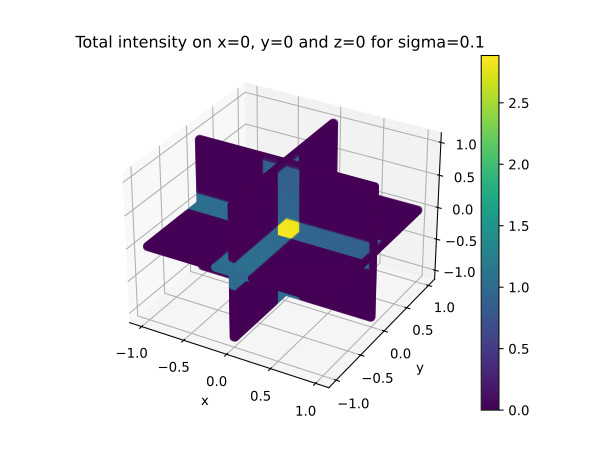
\includegraphics[width=1.0\textwidth]{img/3d_sym_gauss_seidel_0.1.jpg}
    \label{fig:3d_0.1}
    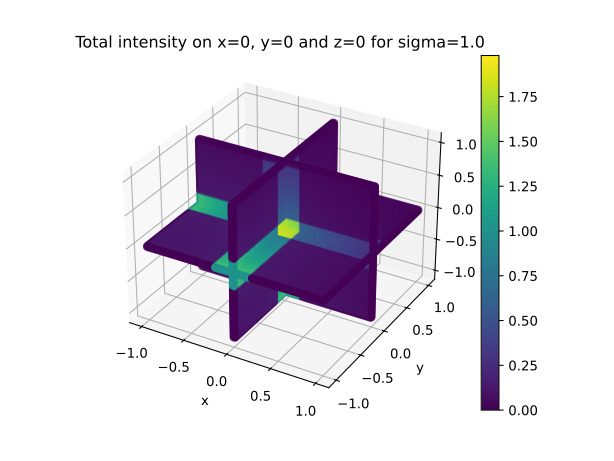
\includegraphics[width=1.0\textwidth]{img/3d_sym_gauss_seidel_1.0.jpg}
    \label{fig:3d_1}
\end{figure}

\begin{figure}[H]
    \centering
    \caption{3D visualization of sum of $F_i$}
    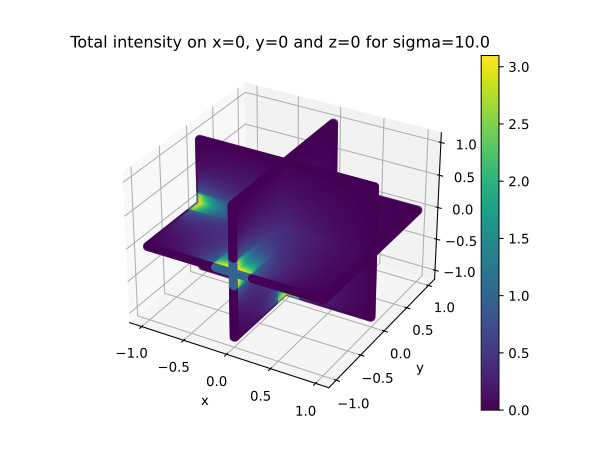
\includegraphics[width=1.0\textwidth]{img/3d_sym_gauss_seidel_10.0.jpg}
    \label{fig:3d_10}
    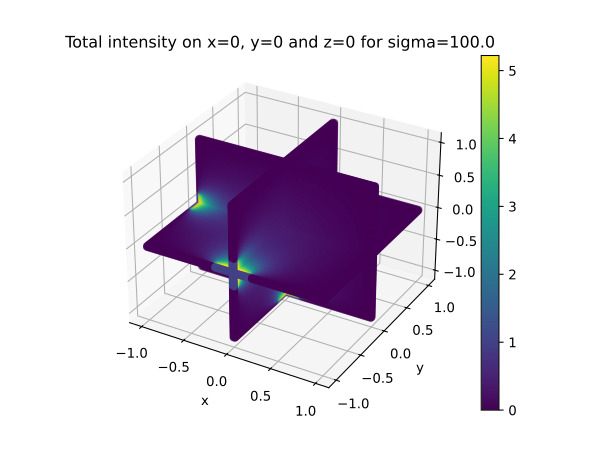
\includegraphics[width=1.0\textwidth]{img/3d_sym_gauss_seidel_100.0.jpg}
    \label{fig:3d_100}
\end{figure}

\begin{figure}[H]
    \caption{SGS solution for $\sigma=0.1$}
    \hspace*{-2cm}\centering
    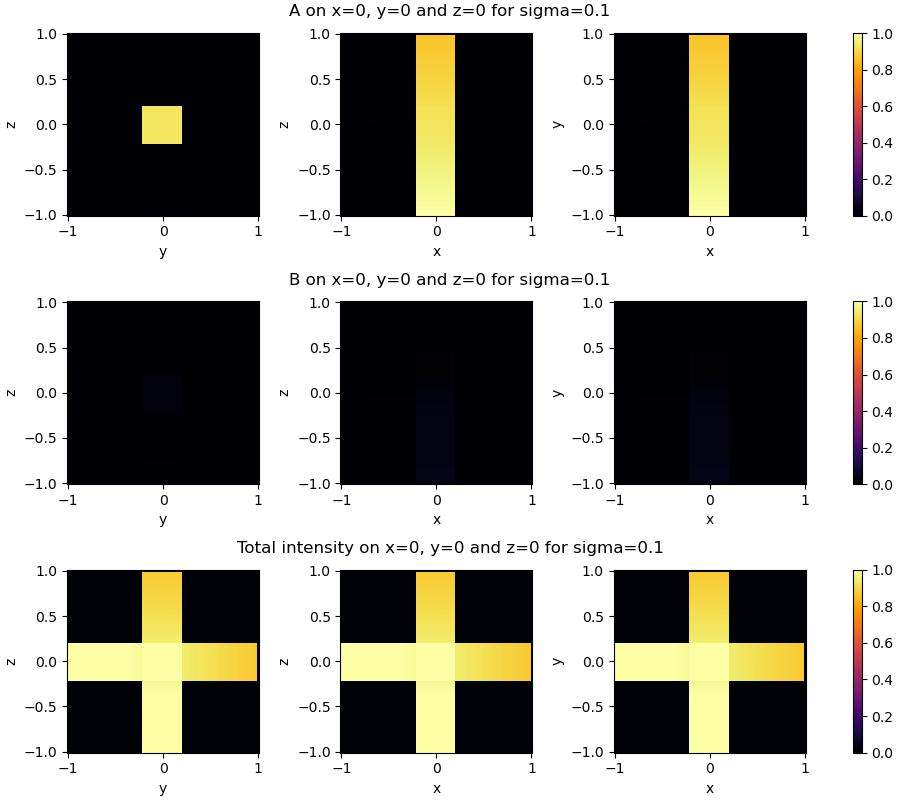
\includegraphics[scale=0.8]{img/2d_sym_gauss_seidel_0.1.jpg}
    \label{fig:sgs_0.1}
\end{figure}

\begin{figure}[H]
    \caption{SGS solution for $\sigma=1$}
    \hspace*{-2cm}\centering
    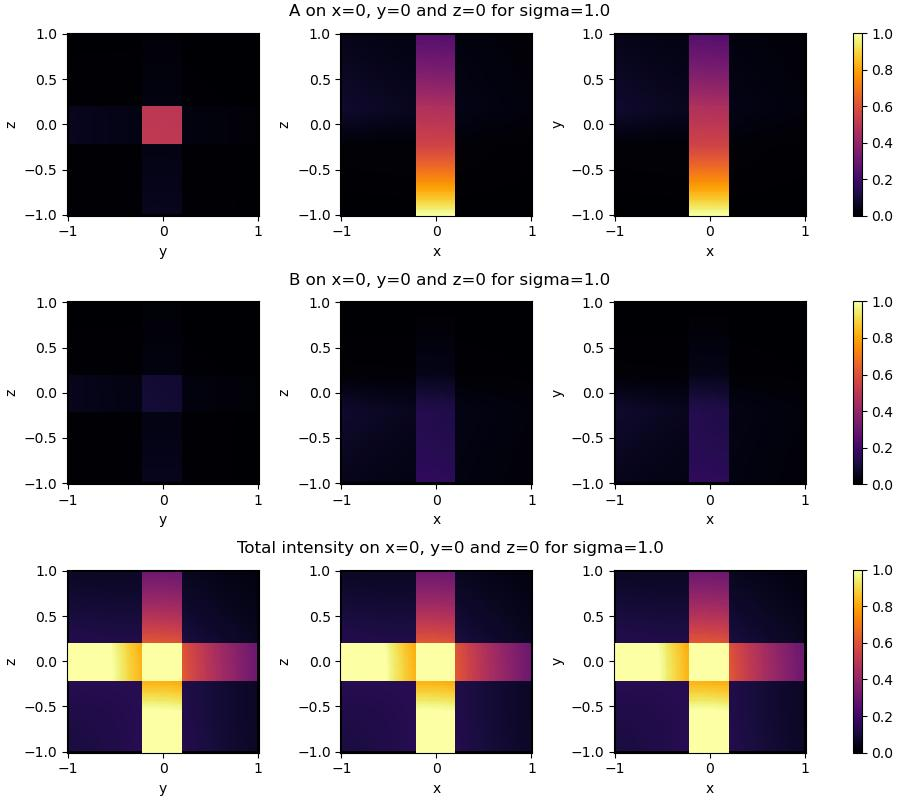
\includegraphics[scale=0.8]{img/2d_sym_gauss_seidel_1.0.jpg}
    \label{fig:sgs_1}
\end{figure}

\begin{figure}[H]
    \caption{SGS solution for $\sigma=10$}
    \hspace*{-2cm}\centering
    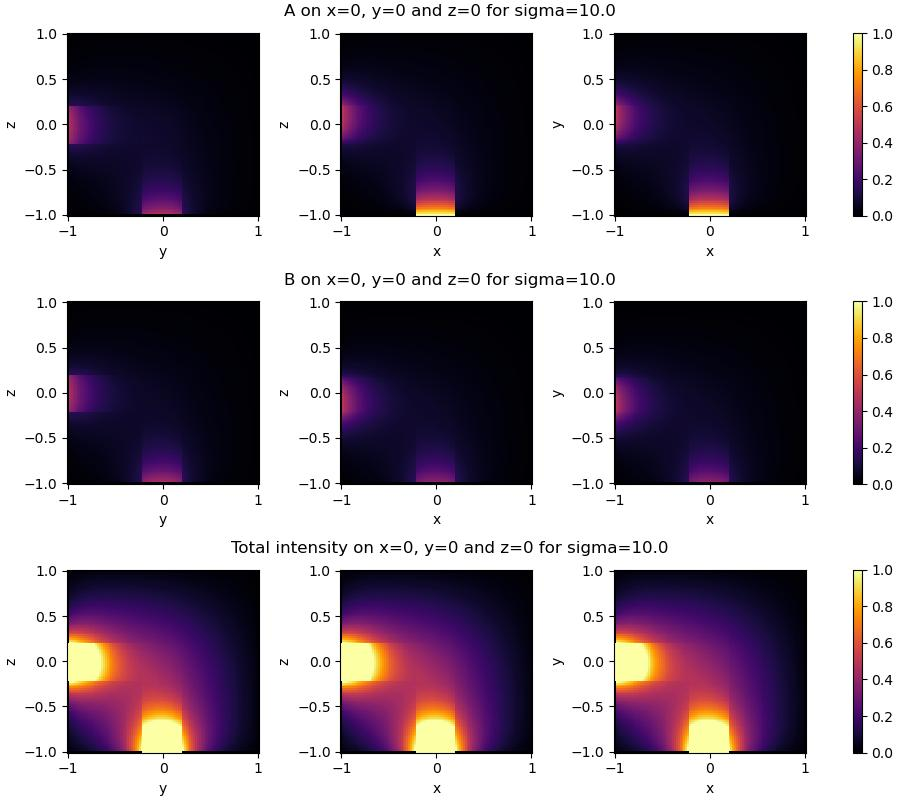
\includegraphics[scale=0.8]{img/2d_sym_gauss_seidel_10.0.jpg}
    \label{fig:sgs_10}
\end{figure}

\begin{figure}[H]
    \caption{SGS solution for $\sigma=100$}
    \hspace*{-2cm}\centering
    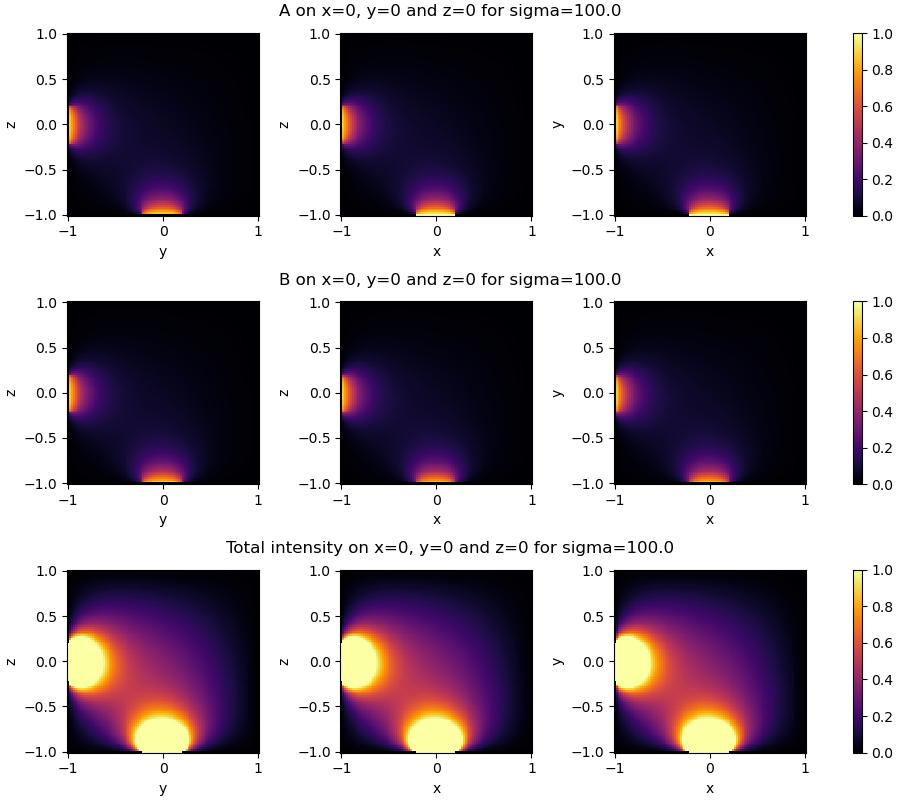
\includegraphics[scale=0.8]{img/2d_sym_gauss_seidel_100.0.jpg}
    \label{fig:sgs_100}
\end{figure}


\section{Conclusion}
\subsection{Revisiting the problem}
This system of PDEs models \href{https://en.wikipedia.org/wiki/Radiative_transfer}{Radiative Transfer}: the physical
phenomenon of energy transfer in the form of electromagnetic radiation (visible light, radio wave etc.). It considers six
velocities in 3D space. $A$ (or $F_1$) denotes the intensity of light transferring in the positive horizontal direction
and $B$ (or $F_2$) in the negative horizontal direction. Similarly, $C$, $D$, $E$ and $F$ denote intensity in their
respective directions. The right-hand side is the scattering term: light is absorbed and emitted in all six directions.
$\sigma$ is the scattering coefficient. The boundary conditions are for light entering through a window from one side in
each direction. With increase in $\sigma$ the decay of intensity along the axes increases and light is scattered more.

\subsection{Solving methods}
Fixed-point (FP) iteration with relaxation and Symmetric Gauss-Seidel (SGS) with successive over-relaxation were employed
to solve the system numerically for various values of $\sigma$. The choice of relaxation is not clear in either case and
would depend on the value of $\sigma$. However, with some experimentation, it can drastically improve the convergence
rate. SGS converges in fewer iterations but FP converges faster due to simpler iteration logic: (0.9s vs 0.2s per
iteration). The algorithms were said to have converged when the residual, the numerical difference between the
approximate left-hand side and the right-hand side (root sum squared), was less than the chosen threshold of $10^{-6}$.

\subsection{Observations}
When $\sigma = 0$, A is constant along x and would be equal to the boundary values. When $\sigma$ is very
large, there's a steep drop in A at the very beginning and continues that way. In other words, the larger the $\sigma$,
greater the decay. This can be observed in Figures \ref{fig:3d_0.1}, \ref{fig:sgs_0.1} and \ref{fig:sgs_1}. It can
also be observed that for large $\sigma$, area outside the axes also light up due to scattering.

Due to symmetry of the problem space and the equations, we have $a(x, y, z) = c(y, x, z) = e(z, y, x)$ and $b(x, y, z) =
d(y, x, z) = f(z, y, x)$. So, the 2D plots plot only intensities $A$, $B$ and the sum total. This could potentially
be exploited for a synthetic SGS method.

\end{document}
